\documentclass[12pt,letterpaper,titlepage]{report}
\usepackage{fontspec}
\defaultfontfeatures{Mapping=tex-text}
\usepackage{xunicode}
\usepackage{xltxtra}
\usepackage{enumitem}
\usepackage{paracol}
\usepackage{tikz}
\usetikzlibrary{circuits.logic.US}
\setmainfont{Times New Roman}
\usepackage{amsmath}
\usepackage{amsfonts}
\usepackage{amssymb}
\usepackage{wrapfig}
\usepackage{graphicx}
\graphicspath{{img/}}
\usepackage[margin=0.65in]{geometry}
\author{Jacob Abel}
\title{%
	Homework 3
	\\\large ECE2504 CRN:82729
}

\begin{document}
\maketitle
\paragraph{Question 1: }(6 pts)\\
\begin{tikzpicture}[scale=0.5, circuit logic US]
\matrix[column sep = 5mm] {
	\node (A){$\overline{A}$}; &				&\\							&\\
					& \node[xor gate](xor1){};	&\\							&\\
	\node (B){$B$}; &							&\\							&\\
					&							&\node[nand gate](nand1){}; &\node (F){$F$};\\
	\node (C){$\overline{C}$}; &				&\\							&\\
					& \node[nor gate](nor1){};	&\\							&\\
	\node (D){$D$}; &							&\\							&\\
};
\draw (A.east) -- ++(right:5mm) |- (xor1.input 1);
\draw (B.east) -- ++(right:5mm) |- (xor1.input 2);
\draw (C.east) -- ++(right:5mm) |- (nor1.input 1);
\draw (D.east) -- ++(right:5mm) |- (nor1.input 2);
\draw (xor1.output) -- ++(right:5mm) |- (nand1.input 1);
\draw (nor1.output) -- ++(right:5mm) |- (nand1.input 2);
\draw (nand1.output) -- ++(right:5mm) |- (F.west);
\end{tikzpicture}
	\begin{enumerate}[label=\alph*)]
	\item Write the logic equation for the variable F in the circuit below, as implemented.\\ 
	$ F = \overline{(\overline{A} \oplus B)  (\overline{\overline{C} + D})} $
	\item Complete the truth table.
	
	\columnratio{0.5}
	\begin{paracol}{3}     
	\switchcolumn
	\def\arraystretch{1.5} 
	\begin{tabular}{|c c|c|}          \hline
	A & B & $\overline{A} \oplus B$ \\\hline
	0 & 0 & 1                       \\\hline
	0 & 1 & 0                       \\\hline
	1 & 0 & 0                       \\\hline
	1 & 1 & 1                       \\\hline
	\end{tabular}\medskip
	
	\begin{tabular}{|c c|c|}                \hline
	A & B & $\overline{\overline{A} + B}$ \\\hline
	0 & 0 & 0                             \\\hline
	0 & 1 & 0                             \\\hline
	1 & 0 & 1                             \\\hline
	1 & 1 & 0                             \\\hline
	\end{tabular}	

	\switchcolumn
	\begin{tabular}{|c c|c|}           \hline
	A & B & $\overline{A} \oplus  B$ \\\hline
	0 & 0 & 1                        \\\hline
	0 & 1 & 1                        \\\hline
	1 & 0 & 1                        \\\hline
	1 & 1 & 0                        \\\hline
	\end{tabular}			
	\switchcolumn	
	\def\arraystretch{1.3} 
	\begin{tabular}{|c c c c|c|c|c|}\hline
	A & B & C & D & $\overline{A} \oplus B$ & $\overline{\overline{A} + B}$ & F \\\hline
	0 & 0 & 0 & 0 & 1 & 0 & 1         \\\hline
	0 & 0 & 0 & 1 & 1 & 0 & 1         \\\hline
	0 & 0 & 1 & 0 & 1 & 1 & 0         \\\hline
	0 & 0 & 1 & 1 & 1 & 0 & 1         \\\hline
	0 & 1 & 0 & 0 & 0 & 0 & 1         \\\hline
	0 & 1 & 0 & 1 & 0 & 0 & 1         \\\hline
	0 & 1 & 1 & 0 & 0 & 1 & 1         \\\hline
	0 & 1 & 1 & 1 & 0 & 0 & 1         \\\hline
	1 & 0 & 0 & 0 & 0 & 0 & 1         \\\hline
	1 & 0 & 0 & 1 & 0 & 0 & 1         \\\hline
	1 & 0 & 1 & 0 & 0 & 1 & 1         \\\hline
	1 & 0 & 1 & 1 & 0 & 0 & 1         \\\hline
	1 & 1 & 0 & 0 & 1 & 0 & 1         \\\hline
	1 & 1 & 0 & 1 & 1 & 0 & 1         \\\hline
	1 & 1 & 1 & 0 & 1 & 1 & 0         \\\hline
	1 & 1 & 1 & 1 & 1 & 0 & 1         \\\hline
	\end{tabular}
	\end{paracol} 
	\pagebreak
	\item Find an equivalent expression in sum‐of‐products form. (Hint: you can check your result by verifying that the truth table remains the same.)
	
	\begin{align*}
	F(A,B,C,D) =\; &\Sigma m(0,1,3,4,5,6,7,8,9,10,11,12,13,15)\\
	F(A,B,C,D) =\; & \overline{A}\;\overline{B}\;\overline{C}\;\overline{D}
	         	   + \overline{A}\;\overline{B}\;\overline{C}\;D
	         	   + \overline{A}\;\overline{B}\;C\;D
	         	   + \overline{A}\;B\;\overline{C}\;\overline{D}
	         	   + \overline{A}\;B\;\overline{C}\;D
	           \\+ & \overline{A}\;B\;C\;\overline{D}
	         	   + \overline{A}\;B\;C\;D
	         	   + A\;\overline{B}\;\overline{C}\;\overline{D}
	         	   + A\;\overline{B}\;\overline{C}\;D
	         	   + A\;\overline{B}\;C\;\overline{D}
	         	   + A\;\overline{B}\;C\;D
	           \\+ & A\;B\;\overline{C}\;\overline{D}
	         	   + A\;B\;\overline{C}\;D
	         	   + A\;B\;C\;D 
	         	   \\
	F(A,B,C,D) =\; & \overline{A}\;\overline{B}\;\overline{C}\;\overline{D}
	         	   + A\;\overline{B}\;\overline{C}\;\overline{D}
	         	   + \overline{A}\;\overline{B}\;\overline{C}\;D
	         	   + A\;\overline{B}\;\overline{C}\;D
	               + \overline{A}\;\overline{B}\;C\;D
	         	   + A\;\overline{B}\;C\;D
	           \\+ & \overline{A}\;B\;\overline{C}\;\overline{D}
	               + A\;B\;\overline{C}\;\overline{D}
	         	   + \overline{A}\;B\;\overline{C}\;D
	         	   + A\;B\;\overline{C}\;D
	         	   + \overline{A}\;B\;C\;D
	           \\+ & A\;B\;C\;D
	         	   + A\;\overline{B}\;C\;\overline{D}
	               + \overline{A}\;B\;C\;\overline{D}
	         	   \\
	F(A,B,C,D) =\; & (\overline{A} + A)
				   ( \overline{B}\;\overline{C}\;\overline{D}
	         	   + \overline{B}\;\overline{C}\;D
	               + \overline{B}\;C\;D
	               + B\;\overline{C}\;\overline{D}
	         	   + B\;\overline{C}\;D
	         	   + B\;C\;D
	         	   )
	           \\+ & A\;\overline{B}\;C\;\overline{D}
	               + \overline{A}\;B\;C\;\overline{D}
	               \\
    F(A,B,C,D) =\; & 
				     \overline{B}\;\overline{C}\;\overline{D}
	               +           B \;\overline{C}\;\overline{D}
	         	   + \overline{B}\;\overline{C}\;D
	         	   +           B \;\overline{C}\;D
	               + \overline{B}\;C\;D
	         	   +           B \;C\;D
	           \\+ & A\;\overline{B}\;C\;\overline{D}
	               + \overline{A}\;B\;C\;\overline{D}
	               \\
    F(A,B,C,D) =\; & (\overline{B} + B) ( 
	               + \;\overline{C}\;\overline{D}
	         	   + \;\overline{C}\;D
	         	   + \;C\;D
	         	   )
	               + A\;\overline{B}\;C\;\overline{D}
	               + \overline{A}\;B\;C\;\overline{D}
	               \\
    F(A,B,C,D) =\; &  
	         	     \overline{C}\;D
	         	   +           C \;D
	               + \overline{C}\;\overline{D}
	               + A\;\overline{B}\;C\;\overline{D}
	               + \overline{A}\;B\;C\;\overline{D}
	               \\
    F(A,B,C,D) =\; & (\overline{C} + C) ( 
	         	   + D
	         	   )
	               + \overline{C}\;\overline{D}
	               + A\;\overline{B}\;C\;\overline{D}
	               + \overline{A}\;B\;C\;\overline{D}
	               \\
    F(A,B,C,D) =\; & 
	         	     D
	               + \overline{C}\;\overline{D}
	               + A\;\overline{B}\;C\;\overline{D}
	               + \overline{A}\;B\;C\;\overline{D}
	               \\
	\end{align*}
	
	\end{enumerate}

\pagebreak
\paragraph{Question 2: }(6 pts)\\
\begin{tikzpicture}[scale=0.5, circuit logic US]
\matrix[column sep = 5mm] {
	\node (A){$A$}; &							&\\							&\\
					&\node[nand gate](nand1){};	&\\							&\\
	\node (B){$\overline{B}$}; &				&\\							&\\
					&							&\node[nand gate](nand2){}; &\node (G){$G$};\\
	\node (C){$C$}; &							&\\							&\\
					& \node[nor gate](nor1){};	&\\							&\\
	\node (D){$D$}; &							&\\							&\\
};
\draw (A.east) -- ++(right:5mm) |- (nand1.input 1);
\draw (B.east) -- ++(right:5mm) |- (nand1.input 2);
\draw (C.east) -- ++(right:5mm) |- (nor1.input 1);
\draw (D.east) -- ++(right:5mm) |- (nor1.input 2);
\draw (nand1.output) -- ++(right:5mm) |- (nand2.input 1);
\draw (nor1.output) -- ++(right:5mm) |- (nand2.input 2);
\draw (nand2.output) -- ++(right:5mm) |- (G.west);
\end{tikzpicture}

\begin{enumerate}[label=\alph*)]
	\item Write the logic equation for the variable F in the circuit below, as implemented. \\
	$ G = \overline{\overline{(A\overline{B})}\;\overline{(C + D)}}$
	\item Complete the truth table. 
	\columnratio{0.5}
	\begin{paracol}{3}     
	\switchcolumn
	\def\arraystretch{1.5} 
	\begin{tabular}{|c c|c|}               \hline
	A & B & $\overline{(A\overline{B})}$ \\\hline
	0 & 0 & 1                            \\\hline
	0 & 1 & 1                            \\\hline
	1 & 0 & 0                            \\\hline
	1 & 1 & 1                            \\\hline
	\end{tabular}\medskip
	
	\begin{tabular}{|c c|c|}       \hline
	A & B & $\overline{(A + B)}$ \\\hline
	0 & 0 & 1                     \\\hline
	0 & 1 & 0                     \\\hline
	1 & 0 & 0                     \\\hline
	1 & 1 & 0                     \\\hline
	\end{tabular}	

	\switchcolumn
	\begin{tabular}{|c c|c|}    \hline
	A & B & $\overline{A\;B}$ \\\hline
	0 & 0 & 1                 \\\hline
	0 & 1 & 1                 \\\hline
	1 & 0 & 1                 \\\hline
	1 & 1 & 0                 \\\hline
	\end{tabular}			
	\switchcolumn	
	\def\arraystretch{1.5} 
	\begin{tabular}{|c c c c|c|c|c|}\hline
	A & B & C & D & $\overline{(A\overline{B})}$ & $\overline{(C + D)}$ & G \\\hline
	0 & 0 & 0 & 0 & 1 & 1 & 0 \\\hline
	0 & 0 & 0 & 1 & 1 & 0 & 1 \\\hline
	0 & 0 & 1 & 0 & 1 & 0 & 1 \\\hline
	0 & 0 & 1 & 1 & 1 & 0 & 1 \\\hline
	0 & 1 & 0 & 0 & 1 & 1 & 0 \\\hline
	0 & 1 & 0 & 1 & 1 & 0 & 1 \\\hline
	0 & 1 & 1 & 0 & 1 & 0 & 1 \\\hline
	0 & 1 & 1 & 1 & 1 & 0 & 1 \\\hline
	1 & 0 & 0 & 0 & 0 & 1 & 1 \\\hline
	1 & 0 & 0 & 1 & 0 & 0 & 1 \\\hline
	1 & 0 & 1 & 0 & 0 & 0 & 1 \\\hline
	1 & 0 & 1 & 1 & 0 & 0 & 1 \\\hline
	1 & 1 & 0 & 0 & 1 & 1 & 0 \\\hline
	1 & 1 & 0 & 1 & 1 & 0 & 1 \\\hline
	1 & 1 & 1 & 0 & 1 & 0 & 1 \\\hline
	1 & 1 & 1 & 1 & 1 & 0 & 1 \\\hline
	\end{tabular}
	\end{paracol} 
	\pagebreak
	\item Find an equivalent expression in product-of-sums form. (Hint: you can check your result by verifying that the truth table remains the same.)
	\begin{align*}
		G(A,B,C,D) =\; &\Pi m(0, 4, 12)
					   \\
		G(A,B,C,D) =\; & (          A +          B +          C +          D )
					     (          A +\overline{B}+          C +          D )
					     (\overline{A}+\overline{B}+          C +          D )
					   \\
		G(A,B,C,D) =\; & (AB'+AC+AD+BA'+BC+C+CD+D)
					     (          A +\overline{B}+          C +          D )
					   \\
		G(A,B,C,D) =\; & (
							AB'+AC+AD+ACD
							+B'D
							+A'BC+C+CD
							+A'BD+D
						 )
					   \\
	\end{align*}
\end{enumerate}
\pagebreak
\paragraph{Question 3: }(3 pts) Use Boolean algebra to prove that $wxy’ +xy’z’ + xy + y’z = x + y’z$
\begin{align*}
wx\overline{y} +x\overline{y}\;\overline{z} + xy + \overline{y}z &= x + \overline{y}z\\
x\overline{y}(w+\overline{z}) + xy + \overline{y}z &= x + \overline{y}z\\
(\overline{y}+y)(x(w+\overline{z}) + 1) + \overline{y}z &= x + \overline{y}z\\
x + \overline{y}z &= x + \overline{y}z\\
\end{align*}
\pagebreak
\paragraph{Question 4: } (10 pts) Given the Boolean function $F = x’y’z’+ x’yz’ + xy’z +xyz$ 
\begin{enumerate}[label=\alph*)]
	\item List the truth table.\\
	\def\arraystretch{1.5} 
	\begin{tabular}{|c c c|c|}\hline
	x & y & z & F \\\hline
	0 & 0 & 0 & 1 \\\hline
	0 & 0 & 1 & 0 \\\hline
	0 & 1 & 0 & 1 \\\hline
	0 & 1 & 1 & 0 \\\hline
	1 & 0 & 0 & 0 \\\hline
	1 & 0 & 1 & 1 \\\hline
	1 & 1 & 0 & 0 \\\hline
	1 & 1 & 1 & 1 \\\hline
	\end{tabular}

	\item Draw the logic diagram using the original Boolean expression. \\
	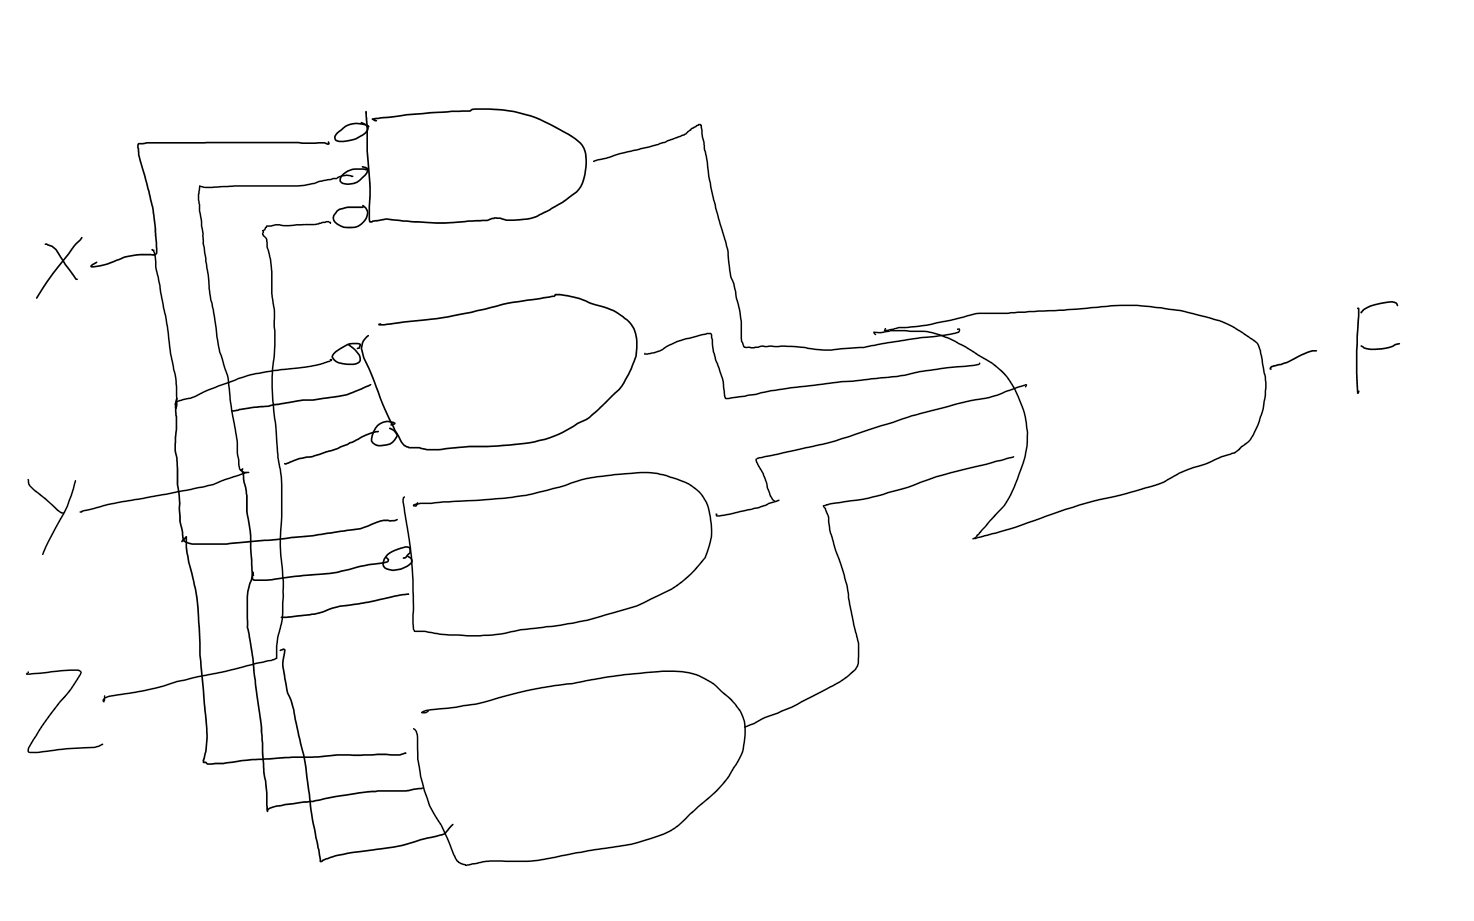
\includegraphics[width=8cm]{hw3p4b}

	\item Simplify using Boolean algebra. 
	\begin{align*}
	F =& x’y’z’+ x’yz’ + xy’z +xyz\\
	F =& (y'+y)(x’z’ + xz)\\
	F =& (x’z’ + xz)
	\end{align*}
\pagebreak
	\item List the truth table of the simplified expression and show it is equivalent to the original. \\
	\def\arraystretch{1.5} 
	\begin{tabular}{|c c c|c|}\hline
	x & y & z & F \\\hline
	0 & 0 & 0 & 1 \\\hline
	0 & 0 & 1 & 0 \\\hline
	0 & 1 & 0 & 1 \\\hline
	0 & 1 & 1 & 0 \\\hline
	1 & 0 & 0 & 0 \\\hline
	1 & 0 & 1 & 1 \\\hline
	1 & 1 & 0 & 0 \\\hline
	1 & 1 & 1 & 1 \\\hline
	\end{tabular}
	\item Draw the logic diagram of the simplified function and compare the total number of gates to part (b). \\
		3 Gates vs 5 Gates\\
		\includegraphics[width=8cm]{hw3p4e}

\end{enumerate}
\pagebreak
\paragraph{Question 5: } (9 pts)  Consider the following Boolean function: $F = A′B′C′ + AB′C + ABC′$ For this question, do not use gates with inverted inputs. If you need an inverter, show it explicitly. 
\begin{enumerate}[label=\alph*)]
	\item Implement it using only NOR gates and inverters? Draw the logic circuit.  Assume your NOR gates can have up to four inputs.
	\begin{align*}
	F =& \overline{A}\;\overline{B}\;\overline{C} + A\overline{B}C + AB\overline{C}
	\\=& \overline{\overline{\overline{A+B+C}} + \overline{\overline{\overline{A}+B+\overline{C}}} + \overline{\overline{\overline{A}+\overline{B}+C}}}
	\end{align*}
	\includegraphics[width=8cm]{hw3p5a}

	\item Redraw the circuit using only 2‐input NOR gates. \\
	Hint: First, convert to 2‐input gates.  Then convert to NORs.  
		\begin{align*}
	F =& \overline{A}\;\overline{B}\;\overline{C} + A\overline{B}C + AB\overline{C}
	\\=& \overline{A}\;(\overline{B+C}) + A((\overline{B+\overline{C}}) + (\overline{\overline{B}+C}))
	\\=& \overline{\overline{A+\overline{(\overline{B+C}))}} + (\overline{\overline{A}+(\overline{(\overline{B+\overline{C}}) + (\overline{\overline{B}+C}))})})}
	\end{align*}
	%\includegraphics[width=8cm]{hw3p5b}
	\item Now implement the function using only NAND gates with up to 4‐inputs. \\
$
	F = \overline{A}\;\overline{B}\;\overline{C} + A\overline{B}C + AB\overline{C}
	  = ( \overline{
				\overline{A}\;\overline{B}\;\overline{C}
			}
		 ) + \overline{(
		 	\overline{
		 		A\overline{B}C
		 	}
		 )} + \overline{(
		 	\overline{
			 	AB\overline{C}
			}
		 })
	  = \overline{(\overline{
		 ( \overline{
				\overline{A}\;\overline{B}\;\overline{C}
			}
		 ) \; \overline{(
		 	\overline{
		 		A\overline{B}C
		 	}
		 )} \; \overline{(
		 	\overline{
			 	AB\overline{C}
			}
		 })
		 })}
$\\
	\includegraphics[width=12cm]{hw3p5c}


\end{enumerate}
\pagebreak
\paragraph{Question 6: } (6 pts)  Consider the following Boolean function:  $F= (x + y + z′) \bullet (x + y′ + z)\bullet (x′ + y′ + z′) $For this question, do not use gates with inverted inputs. If you need an inverter, show it explicitly. 
\begin{enumerate}[noitemsep, label=\alph*)]
	\item Implement it using only NAND gates and inverters? Draw the logic circuit.  Assume your NAND gates can have 
up to four inputs.
	\begin{align*}
	F =& (x + y + z′) \bullet (x + y′ + z)\bullet (x′ + y′ + z′)
	\\=& \overline{(x'y'z)}\bullet\overline{(x'yz')}\bullet\overline{(xyz)}
	\\=& \overline{\overline{({\overline{\overline{(x'y'z)}} \bullet \overline{\overline{(x'yz')}}\bullet \overline{\overline{(xyz)}})}}}
	\end{align*}
	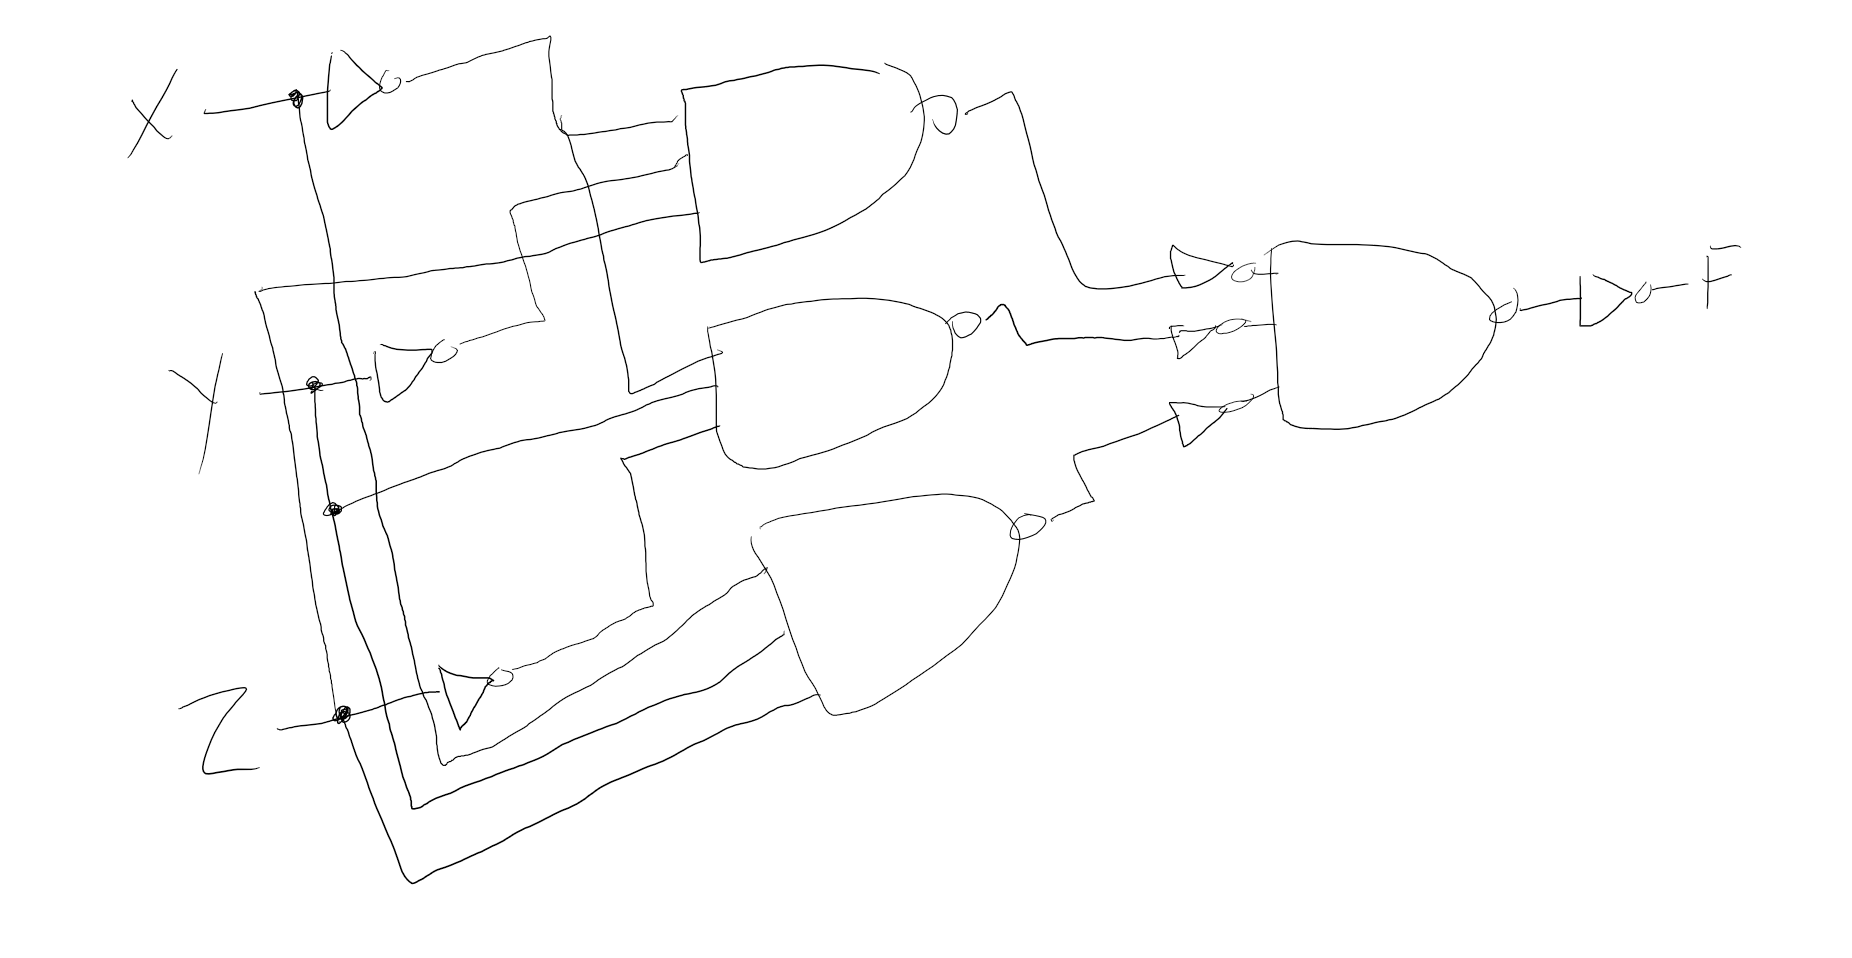
\includegraphics[width=12cm]{hw3p6a}
	\item Redraw the circuit using only 2‐input NAND gates. \\
	Hint: First, convert to 2‐input gates.  Then convert to NANDs.

\end{enumerate}
\pagebreak
\paragraph{Question 7: } (3 pts) Derive a Boolean expression for the complement G’ of the function $G(a,b,c) = a′bc′ + a′c + ab′c′$. Simplify.  
\begin{align*}
G(a,b,c) =& a′bc′ + a′c + ab′c′\\
\overline{G}(a,b,c) =& (a+b'+c)(a+c')(a'+b+c)
				    \\
				  	=& (a+b'+c)(a+c')(a'+b+c)
				    \\
				  	=& (
				  		a'b'c'+a'c'
				  		+ab+abc+abc'+bc'
				  		+ac+ab'c			  		
				  		)
				    \\
				  	=& (
				  		a'b'c'+a'c'
				  		+ab+bc'+ac+ab'c
				  		)
\end{align*}
\bigskip\noindent
GRADING SCALE\\\medskip
Total: 43 pts\bigskip
\begin{flushleft}
\def\arraystretch{1.5}
\begin{tabular}{ | l | c | c | c | c | c | c | c | c | } \hline
Pts          & 0  & 5  & 10 & 15 & 21 & 26 & 32 & 37     \\\hline
Letter Grade & D- & D  & C- & C  & B- & B  & A- & A      \\\hline
\end{tabular}
\end{flushleft}
\end{document}
